
\chapter{الهندسة الهذلولية (الزائدية)}
\section[مقدمة]{مقدمة \cite{ref3}}

الهندسة الهذلولية (الزائدية) هي إحدى الهندسات اللاإقليدية، وقد قام بتأسيسها وتطويرها كلٌّ من العالمين János Bolyai الهنغاري و Nikolai Lobachevsky الروسي في الفترة ما بين (1820--1830م). وقد تم ذلك عبر أخذ نقيض بديهية بليفير (وهي إحدى المكافئات لبديهية التوازي عند إقليدس)، والتي تنص على ما يلي:

من نقطة لا تقع على مستقيم معلوم يمكن رسم أكثر من مستقيم موازٍ لذلك المستقيم.

وبهذا أصبحت الهندسة الهذلولية (الزائدية) نظامًا بديهيًا يعتمد على البديهيات الأربع الأولى لهندسة إقليدس، بالإضافة إلى بديهية إضافية تناقض بديهية التوازي الإقليدية، وتسمى هذه البديهية \textbf{بديهية التوازي الزائدية} أو \textbf{البديهية المميزة للهندسة الهذلولية (الزائدية)}.

بعد المحاولات العديدة لإثبات بديهية التوازي الخامسة لإقليدس، بدأ العلماء يشكّون في إمكانية اشتقاقها من البديهيات الأخرى. ونتيجة لذلك ظهرت الهندسة اللاإقليدية، حيث تم إثبات استقلالية هذه البديهية عن باقي بديهيات إقليدس، وبالتالي تم بناء هندسات جديدة على أساس بديهيات إقليدس مع استبدال أو حذف البديهية الخامسة.

وقد أثبت كل من János Bolyai و Nikolai Lobachevsky أن البديهية الخامسة مستقلة عن البديهيات الأربع الأولى، وذلك عبر استبدالها بنقيضها الذي ينص على:

يوجد أكثر من مستقيم موازٍ لمستقيم معين يمر بنقطة خارجه.

وتسمى هذه الهندسة الناتجة \textbf{الهندسة الهذلولية (الزائدية)}.

\begin{axiom}[التوازي الهذلولية (HPP)]
	إذا كان $m$ مستقيمًا و $P$ نقطة خارجه، فإنه يوجد على الأقل شعاعان $\overrightarrow{PR}$ و $\overrightarrow{PS}$ بحيث:
	\begin{enumerate}
		\item الشعاعان $\overrightarrow{PR}$ و $\overrightarrow{PS}$ غير متعاكسين.
		\item الشعاعان $\overrightarrow{PR}$ و $\overrightarrow{PS}$ لا يشتركان مع المستقيم $m$.
		\item الشعاع $\overrightarrow{PQ}$ يقطع المستقيم $m$ إذا وفقط إذا كان يقع بين الشعاعين $\overrightarrow{PR}$ و $\overrightarrow{PS}$.
	\end{enumerate}
\end{axiom}

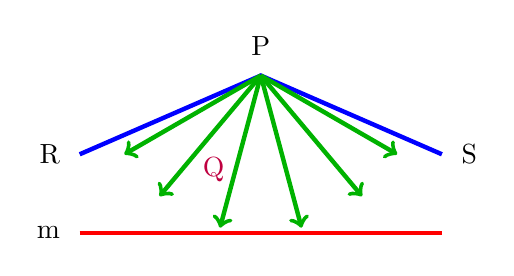
\begin{tikzpicture}[ultra thick]
	
	\coordinate (P) at (0, 2);
	\coordinate (R) at (-2.3, 1);
	\coordinate (S) at (2.3, 1);
	\coordinate (M_start) at (-2.3, 0);
	\coordinate (M_end) at (2.3, 0);
	
	% Triangle sides in blue
	\draw[blue] (R) -- (P) -- (S);
	
	% Base line in red
	\draw[red] (M_start) -- (M_end);
	
	% Arrows in green
	\foreach \angle/\len in {210/2, 230/2, 255/2, 285/2, 310/2, 330/2} {
		\draw[->, green!70!black] (P) -- ++(\angle:\len);
	}
	
	% Labels in black (or customize individually)
	\node[above=3pt, black] at (P) {P};
	\node[left=3pt, black] at (R) {R};
	\node[right=3pt, black] at (S) {S};
	\node[left=3pt, black] at (M_start) {m};
	
	% Highlight Q in purple
	\node[purple] at (-0.6, 0.8) {Q};
	
\end{tikzpicture}

وتعني هذه البديهية أنه يمكن رسم أكثر من مستقيم موازٍ لمستقيم معلوم يمر من نقطة خارجه، وهو ما يمثل نقيض بديهية التوازي الإقليدية الخامسة.

\begin{definition}
	يُسمّى الشعاعان $\overrightarrow{PR}$ و $\overrightarrow{PS}$ الواردان في بديهية (HPP) بالشعاعين المتوازيين للمستقيم $m$ من النقطة $P$.
	
	ولغرض تمثيل الهندسة الهذلولية باستخدام مفاهيم الهندسة الإقليدية، توجد عدة نماذج، من أهمها:
	
	\begin{enumerate}
		\item \textbf{نموذج كلاين (Klein Model):} \\
		ينص نموذج كلاين على أن المستوى الهذلولي هو مجموعة النقاط الداخلية لدائرة في المستوى الإقليدي، وأن مستقيمات هذا المستوى هي أوتار هذه الدائرة، بحيث يُقصد بالوتر المفتوح الجزء الداخلي فقط دون نقاط محيط الدائرة.
	
يلاحظ أن المستقيمات التي تمر بالنقطة $P$ لا تشتركان مع المستقيم $n$ حسب تعريف التوازي الهذلولي وحقيقة أنهما يلتقيان خارج الدائرة لا تهمنا وذلك لأنها تقع خارج المستوي الهذلولي.

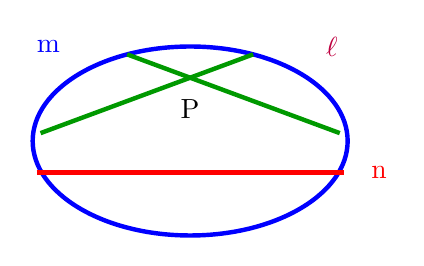
\begin{tikzpicture}[ultra thick]
	
	% Ellipse in blue
	\draw[blue] (0,0) ellipse (2cm and 1.2cm);
	
	% Lines
	\draw[red] (-1.95, -0.4) -- (1.95, -0.4);          % horizontal line
	\draw[green!60!black] (-1.9, 0.1) -- (0.8, 1.1);    % left diagonal
	\draw[green!60!black] (1.9, 0.1) -- (-0.8, 1.1);    % right diagonal
	
	% Labels
	\node[black] at (0, 0.4) {P};
	\node[blue] at (-1.8, 1.2) {m};
	\node[purple] at (1.8, 1.2) {$\ell$};
	\node[red] at (2.4, -0.4) {n};
	
\end{tikzpicture}

\item \textbf{نموذج بون كيري (بونكارية) Poincare Model:}\\ النموذج الذي قدمه ينص على اعتبار المستقيمات (الخطوط) هي أقواس مفتوحة من الدوائر المعامدة للدائرة التي تمثل المستوي الهذلولي. تكون دائرتان متعامدتان إذا كانت أنصاف أقطار كل منهما المارة بنقطتي التقاطع متعامدة.

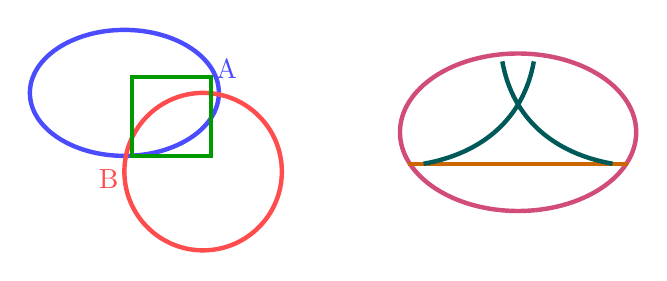
\begin{tikzpicture}[ultra thick]
	
	% Left figure
	\begin{scope}[shift={(0,0)}]
		% Ellipse
		\draw[blue!70] (0,0.5) ellipse (1.2 and 0.8);
		
		% Circle
		\draw[red!70] (1,-0.5) circle (1);
		
		% Square
		\draw[green!60!black] (0.1,-0.3) -- (1.1,-0.3) -- (1.1,0.7) -- (0.1,0.7) -- cycle;
		
		% Labels
		\node[blue!70] at (1.3,0.8) {A};
		\node[red!70] at (-0.2,-0.6) {B};
	\end{scope}
	
	% Right figure
	\begin{scope}[shift={(5,0)}]
		% Outer ellipse
		\draw[purple!70] (0,0) ellipse (1.5 and 1);
		
		% Base line
		\draw[orange!80!black] (-1.4,-0.4) -- (1.4,-0.4);
		
		% Curves
		\draw[teal!70!black] (-1.2,-0.4) to[out=10,in=-100] (0.2,0.9);
		\draw[teal!70!black] (1.2,-0.4) to[out=170,in=-80] (-0.2,0.9);
	\end{scope}
	
\end{tikzpicture}
\end{enumerate}
\end{definition}

\begin{definition}
	كل من الشعاعين $\overrightarrow{PR}$ و $\overrightarrow{PS}$ المذكورين في (HPP) يُدعى شعاعًا موازيًا للمستقيم $m$ من النقطة $P$.
\end{definition}

\begin{theorem}
	إذا كان شعاع يقع بين شعاع موازٍ لمستقيم معلوم وشعاع يقطع ذلك المستقيم، فإن هذا الشعاع يقطع المستقيم المعلوم.
\end{theorem}
\begin{proof}
	ليكن $\overrightarrow{PR}$ و $\overrightarrow{PS}$ شعاعين موازين للمستقيم $m$ من النقطة $P$. ولتكن $B$ نقطة على المستقيم $m$، وليكن $\overrightarrow{PQ}$ شعاعًا يقع بين $\overrightarrow{PR}$ و $\overrightarrow{PB}$.\\
	نريد إثبات أن $\overrightarrow{PQ}$ يقطع المستقيم $m$.\\
	بما أن $\overrightarrow{PB}$ يقطع المستقيم $m$، فإن الشعاعين $\overrightarrow{PR}$ و $\overrightarrow{PS}$ يقعان على جهتين متقابلتين بالنسبة للمستقيم $\overrightarrow{PB}$. وبما أن $\overrightarrow{PQ}$ يقع بين $\overrightarrow{PR}$ و $\overrightarrow{PB}$، فإنه وفقًا لمبرهنة (Th 47) يقع أيضًا بين $\overrightarrow{PR}$ و $\overrightarrow{PS}$.\\
	وبحسب بديهية التوازي الزائدية (HPP)، فإن كل شعاع يقع بين الشعاعين الموازيين $\overrightarrow{PR}$ و $\overrightarrow{PS}$ يقطع المستقيم $m$، وبالتالي فإن $\overrightarrow{PQ}$ يقطع $m$.\\
	وبنفس الطريقة، إذا كان $\overrightarrow{PQ}$ يقع بين $\overrightarrow{PS}$ و $\overrightarrow{PB}$ فإنه يقطع المستقيم $m$.
\end{proof}


\begin{note}توضح المبرهنة التالية أن المستقيم الموازي هو أول هذه المستقيمات من حيث البنية الهندسية.
\end{note}

\begin{theorem}
	إذا كان $\overrightarrow{PQ}$ لا يقطع المستقيم $m$، ولكن كل شعاع يقع بين $\overrightarrow{PQ}$ و $\overrightarrow{PB}$ (حيث $B$ نقطة على $m$) يقطع المستقيم $m$، فإن $\overrightarrow{PQ}$ يوازي المستقيم $m$.
\end{theorem}

\begin{proof}
	ليكن $m$ مستقيماً ، $P$ نقطة لا تقع على $m$ ، $\overrightarrow{PQ}$ شعاع لا يقطع $m$\\
	من HPP: لا يوجد شعاعان 
	$\overrightarrow{PR}, \overrightarrow{PS}$ من $P$ ويوازيان $m$. لتكن $B$ اية نقطة على $m$\\
	من الفرض: $P, B, Q$ لا تقع على مستقيم واحد\\
	$Q$ لا تقع على المستقيم $\overrightarrow{PB}$\\
	$Q$ تقع في احدى جهتي $PB$\\
من HPP : $\overrightarrow{PR}, \overrightarrow{PS}$ في الجهتين المعاكستين للمستقيم $PB$\\
وعليه يوجد احتمالين 
\begin{enumerate}
	\item اما تقع $Q$ في جهة $\overrightarrow{PB}$ التي تحوي $R$
	\item او تقع $Q$ في حهة $PB$ التي تحوي $S$
\end{enumerate}
\textbf{الاحتمال الأول}: اما تقع $Q$ في جهة $\overrightarrow{PB}$ التي تحوي $R$\\
وهذا يؤدي الى ثلاث احتمالات
\begin{enumerate}[label*=\textbf{\xslalph* -}]
	\item اما $\overrightarrow{PR}$ يقع بين $\overrightarrow{PB}$ و $\overrightarrow{PQ}$
	\item او $\overrightarrow{PQ}$ يقع بين $\overrightarrow{PB}$ و $\overrightarrow{PR}$
	\item او $\overrightarrow{PR}  = \overrightarrow{PQ}$ 
\end{enumerate}
في حالة (أ) : $\overrightarrow{PR}$ يقع بين $\overrightarrow{PB}$ و $\overrightarrow{PQ}$\\
فمن الفرض : 
$\overrightarrow{PR}$ يقطع $m$ وهذا يخالف بديهية التوازي الهذلولية\\
في حالة ب : $\overrightarrow{PQ}$ يقع بين $\overrightarrow{PB}$ و $\overrightarrow{PR}$\\
حسب Th102 : 
$\overrightarrow{PQ}$ يقطع $m$ وهذا يخالف الفرض\\
وعليه الحالة الوحيدة المقبولة عندما $\overrightarrow{PR}  = \overrightarrow{PQ}$\\
وبنفس الطريقة اذا كانت $Q$ تقع في جهة $\overrightarrow{PB}$ التي تحوي $S$
\end{proof}
\begin{theorem}
	إذا كانت النقطة $Q$ هي قدم العمود النازل من النقطة $P$ على المستقيم $m$، وكان $\overrightarrow{PR}$ و $\overrightarrow{PS}$ هما الشعاعان الموازيان للمستقيم $m$ من النقطة $P$، فإن الزاويتين $\angle SPQ$ و $\angle RPQ$ زاويتان حادتان.
\end{theorem}
\begin{proof}
يجب ان نبرهن ان:\\
$\angle 1, \angle 2$ اقل من 90 (زاوية حادة)\\
حسب Th62 : يتحقق واحد فقط مما يلي:
\begin{enumerate}
	\item $\angle 1, \angle 2$ قوائم
	\item $\angle 1, \angle 2$ منفرجة
	\item $\angle 1, \angle 2$ حادة
\end{enumerate}
وحسب البديهية : جميع الزوايا القائمة متساوية\\
اذن 
$\angle 1 = \angle 2$ اذن $\angle 1  \cong \angle 2$\\
اذن الزاويتان 
$\angle 1, \angle 2$ متكاملتان ومتجاورتان\\
وحسب النتيجة و Th58 : $\angle 1, \angle 2$ يكوّنان زوج خطي\\
اذن $\overrightarrow{PQ}$ و $\overrightarrow{PS}$ متعاكسين وهذا تناقض مع Ax17\\
اذن الاحتمال الأول مرفوض\\
الاحتمال الثاني : $\angle 1, \angle 2$ منفرجة\\
اذن 
$\angle 2  > 90$\\
وحسب تعريف العلاقة $<$ : يوجد شعاع $\overrightarrow{PE}$ داخل $\angle 2$ بحيث $\angle 3$ قائمة.\\
$\angle 3, \angle 4$ قوائم\\
اذن مجموعهما 180\\
حسب Th74 : نحصل على $\overrightarrow{PE}$ يوازي $m$ ...... (1).\\
ولكن الشعاع $\overrightarrow{PE}$ يقع بين القاطع $\overrightarrow{PQ}$ والموازي $\overrightarrow{PR}$ (لأنه داخل $\angle 2 $).\\
وحسب Th102 : الشعاع $\overrightarrow{PE}$ يقطع الخط $m$\\
ولكن الخط $PE$ يقطع الخط $m$ ........ (2).\\
من (1) و (2) نحصل على تناقض\\
اذن الاحتمال الثاني مرفوض\\
اذن الاحتمال الوحيد المقبول هو : 
$\angle 1, \angle 2$ حادتان
 \end{proof}

\begin{theorem}
	إذا كان الشعاع $\overrightarrow{PS}$ موازيًا للمستقيم $m$ من النقطة $P$، وكانت $X$ نقطة على الشعاع $\overrightarrow{PS}$ بحيث تقع على الترتيب $P - X - S$، فإن:\\
	\begin{tasks*}
		\item لا يمكن أن يكون الشعاع $\overrightarrow{PX}$ موازيًا للمستقيم $m$.
		\item لا يمكن أن يكون الشعاع $\overrightarrow{PX}$ قاطعًا للمستقيم $m$.
		\item الشعاع $\overrightarrow{PS}$ لا يقطع المستقيم $m$.
	\end{tasks*}
\end{theorem}

\begin{definition}
	ليكن $\overrightarrow{PR}$ و $\overrightarrow{QS}$ شعاعين غير واقعين على مستقيم واحد، ولتكن $P$ و $Q$ نقطتين مختلفتين. يُقال إن الشعاعين $\overrightarrow{PR}$ و $\overrightarrow{QS}$ في نفس الاتجاه إذا وفقط إذا كانا في نفس الجهة بالنسبة للمستقيم $PQ$.
\end{definition}

\begin{theorem}
	إذا كان $\overrightarrow{AR} \parallel \overrightarrow{BS}$ فإن $\overrightarrow{BS} \parallel \overrightarrow{AR}$.
\end{theorem}

\begin{theorem}
	إذا كان شعاعان في نفس الاتجاه ويوازيان شعاعًا ثالثًا، فإن أحدهما يوازي الآخر.
\end{theorem}

\section[المثلث الهذلولي (الزائدي)]{المثلث الهذلولي (الزائدي) \cite{ref4}}

\begin{definition}
	إذا كان الشعاعان $\overrightarrow{XP}$ و $\overrightarrow{YS}$ شعاعين متوازيين، وكان المستقيم $m$ يقطعهما في النقطتين $A$ و $B$ بحيث تقع النقاط على الترتيب $X-A-P$ و $Y-B-S$، فإن اتحاد الشعاعين $\overrightarrow{AP}$ و $\overrightarrow{BS}$ مع القطعة المستقيمة $AB$ يُسمى \textbf{المثلث الهذلولي} أو \textbf{المثلث ذو الرأسين (Two-Vertices Triangle, T.V.T)}، ويرمز له بـ $PABS$.
	
	\begin{tikzpicture}[ultra thick]
		
		\coordinate (X) at (1,3);
		\coordinate (P) at (7,2.3);
		\coordinate (Y) at (0.3,1);
		\coordinate (S) at (7,1);
		\coordinate (topM) at (3.5,4.3);
		\coordinate (botM) at (2.8,-1);
		
		% Lines
		\draw[blue!70] (X) -- (P);
		\draw[red!70] (Y) -- (S);
		\draw[green!60!black] (botM) -- (topM);
		
		% Intersections
		\coordinate (A) at (intersection of X--P and botM--topM);
		\coordinate (B) at (intersection of Y--S and botM--topM);
		
		% Labels
		\node[above left, blue!70] at (A) {A};
		\node[below left, red!70] at (B) {B};
		
		\node[above=3pt, left, blue!70] at (X) {X};
		\node[above=3pt, right, blue!70] at (P) {P};
		
		\node[above=3pt, left, red!70] at (Y) {Y};
		\node[above=3pt, right, red!70] at (S) {S};
		
		\node[above=3pt, green!60!black] at (topM) {m};
		
		% Angles (colored to match lines)
		\pic[draw=blue!70, angle radius=6mm] {angle = X--A--botM};
		\pic[draw=blue!70, angle radius=4mm] {angle = B--A--P};
		
		\pic[draw=red!70, angle radius=4mm]  {angle = A--B--Y};
		\pic[draw=red!70, angle radius=6mm] {angle = S--B--A};
		
	\end{tikzpicture}
	\begin{enumerate}[label=$\bullet$, leftmargin=*]
		\item القطعة المستقيمة $AB$ تسمى ضلع المثلث (T.V.T).
		\item الزاويتان $\angle BAP$ و $\angle ABS$ تسميان الزوايا الداخلية للمثلث.
		\item النقطتان $A$ و $B$ هما رأسا المثلث.
		\item الزاويتان $\angle XAB$ و $\angle YBA$ تسميان الزوايا الخارجية للمثلث.
		\item الزوايا الداخلية والخارجية غير المتجاورة تسمى زوايا متبادلة.
		\item داخل المثلث (T.V.T) هو مجموعة النقاط التي تقع في جهة من $AB$ تحتوي $P$، وفي جهة من $\overrightarrow{AP}$ تحتوي $B$، وفي جهة من $\overrightarrow{BS}$ تحتوي $A$.
		\item النقاط الخارجية هي جميع النقاط التي لا تنتمي إلى الداخل ولا تقع على المثلث.
	\end{enumerate}
\end{definition}

\begin{theorem}
	اذا كان الشعاع 
	$\overrightarrow{PB}$ يقع بين $\overrightarrow{PR}$ و $\overrightarrow{PS}$ وكان $\overrightarrow{PQ}$ يقع بين $\overrightarrow{PB}$ و $\overrightarrow{PR}$ فإن $\overrightarrow{PQ}$ يقع بين الشعاعين $\overrightarrow{PS} , \overrightarrow{PR}$.
\end{theorem}

\begin{theorem}
	\begin{tasks}
		\item المستقيم المار بنقطة داخلية من المثلث (T.V.T) $RABS$ وأحد رؤوسه يقطع الشعاع المقابل لذلك الرأس.
		
		\item المستقيم المار بنقطة داخلية من المثلث $RABS$ ويوازي أحد شعاعيه يقطع ضلع المثلث.
	\end{tasks}
\end{theorem}
\begin{proof}
\begin{tasks*}
	\item نفرض ان P نقطة داخلية للمثلث RABS\\
	اذا كان المستقيم m يمر بالرأس B\\
	فأنه من المبرهنة 57 : الشعاع $\overrightarrow{BP}$ يقطع الشعاع $\overrightarrow{AR}$ وكذلك اذا كان المستقيم يمر بالرأس A\\
	فأنه من المبرهنة 57 : الشعاع 
	$\overrightarrow{AP}$ يطقع الشعاع $\overrightarrow{BS}$

	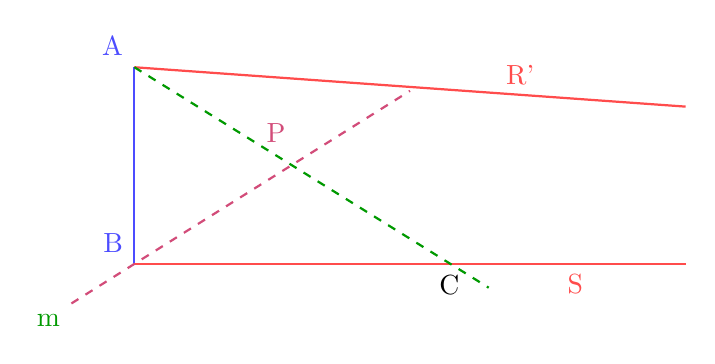
\begin{tikzpicture}[ultra thick]
		
		\coordinate (A) at (0,3.5);
		\coordinate (B) at (0,1);
		\coordinate (C) at (4,1);
		\coordinate (R) at (7,3);
		\coordinate (S) at (7,1);
		\coordinate (m) at (-0.8,0.5);
		\coordinate (P) at (1.8,2.4);
		
		% Main segments
		\draw[thick, blue!70] (A) -- (B);
		\draw[thick, red!70] (A) -- (R) node[pos=0.7, above, red!70] {R'};
		\draw[thick, red!70] (B) -- (S) node[pos=0.8, below, red!70] {S};
		
		% Dashed auxiliary lines
		\draw[dashed, thick, green!60!black] (A) -- (4.5, 0.7);
		\draw[dashed, thick, purple!70] (m) -- (3.5, 3.2);
		
		% Labels
		\node[above left, blue!70] at (A) {A};
		\node[above left, blue!70] at (B) {B};
		\node[below, black] at (C) {C};
		\node[above, purple!70] at (P) {P};
		\node[below left, green!60!black] at (m) {m};
		
	\end{tikzpicture}
	\item نفرض ان النقطة P نقطة داخلية للمثلث RABS\\
	وكذلك المستقيم $\overleftrightarrow{PD}$ يوازي احد الشعاعين وليكن
	$\overrightarrow{BS}$\\
	من مبرهنة 112 (A) : الشعاع $\overrightarrow{AP}$ يقطع الشعاع $\overrightarrow{BS}$ في نقطة مثل C\\
	اذن المستقيم PD يقطع AC في نقطة P\\
	اذن من بديهية باش : المستقيم PD اما ان يقطع الضلع BC او الضلع AB ولكن من الفرض PD لا يقطع الضلع BC \\
	اذن يقطع الضلع AB.\\
	
	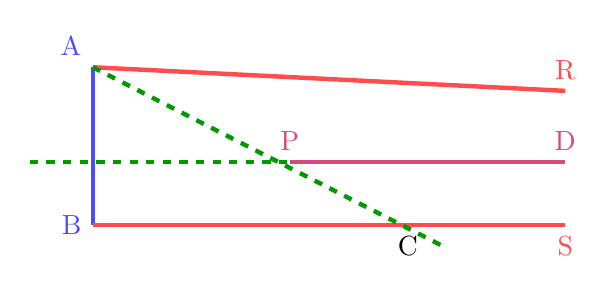
\begin{tikzpicture}[ultra thick]
		
		\coordinate (A) at (0,3);
		\coordinate (B) at (0,1);
		\coordinate (R) at (6,2.7);
		\coordinate (S) at (6,1);
		\coordinate (D) at (6,1.8);
		\coordinate (P) at (2.5,1.8);
		\coordinate (C) at (4,1);
		\coordinate (left_dash) at (-0.8,1.8);
		
		% Main structure
		\draw[blue!70] (A) -- (B);
		\draw[red!70] (A) -- (R);
		\draw[red!70] (B) -- (S);
		
		% Middle segment
		\draw[purple!70] (P) -- (D);
		
		% Auxiliary dashed lines
		\draw[dashed, green!60!black] (left_dash) -- (P);
		\draw[dashed, green!60!black] (A) -- (4.5,0.7);
		
		% Labels
		\node[above left, blue!70] at (A) {A};
		\node[left, blue!70] at (B) {B};
		
		\node[above, red!70] at (R) {R};
		\node[below, red!70] at (S) {S};
		\node[above, purple!70] at (D) {D};
		
		\node[above, purple!70] at (P) {P};
		\node[below, black] at (C) {C};
		
	\end{tikzpicture}
\end{tasks*}
\end{proof}

\begin{theorem}
	\begin{tasks}
		\item المستقيم الذي لا يمر بأي رأس من رؤوس المثلث (T.V.T) $RABS$ ويقطع أحد الشعاعين فإنه يقطع الشعاع الآخر أو ضلع المثلث.\\
		\item المستقيم الذي لا يمر بأي رأس من رؤوس المثلث $RABS$ ويقطع الضلع ولا يوازي أي شعاع فإنه يقطع أحد الشعاعين.
	\end{tasks}
	\begin{proof}
\begin{tasks*}
	\item نفترض أن المستقيم $m$ يقطع الشعاع $\overrightarrow{AR}$ في نقطة مثل $C$\\
	$\therefore$ المستقيم $m$ لا يمر بأي من الرؤوس\\
	$\therefore$ المستقيم $m$ لا يمكن أن يكون نفس المستقيم $BC$\\
	$\therefore$ داخل المثلث مجموعة غير خالية\\
	$\therefore$ توجد نقطة $D$ داخل المثلث $RABS$ تقع على المستقيم $m$ لذلك نحصل على احتمالات لوقوع النقطة $D$\\
	إذا كانت $D$ داخل الزاوية $RCB$ ← فإن الشعاع $CD$ يقع بين الشعاعين $CR$ و $BC$\\
	$\therefore$ من مبرهنة (62) الشعاع $CR$ يوازي الشعاع $BS$\\
	$\therefore$ من مبرهنة (57) المستقيم $m$ يقطع الشعاع $BS$\\
	إذا كانت $D$ داخلية للمثلث $ABC$\\
	$\therefore$ حسب مبرهنة (31) المستقيم $m$ يقطع الضلع $AB$
	
	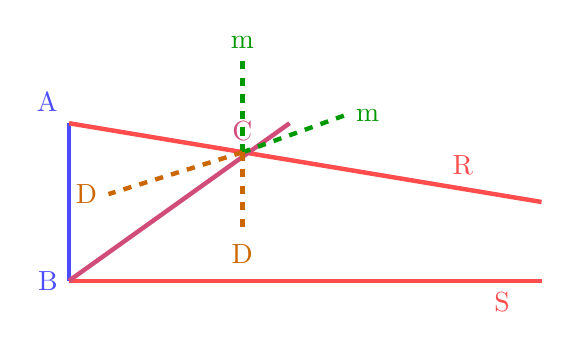
\begin{tikzpicture}[ultra thick]
		
		\coordinate (A) at (0,3);
		\coordinate (B) at (0,1);
		\coordinate (R) at (6,2);
		\coordinate (S) at (6,1);
		\coordinate (C) at (2.2,2.63);
		
		% Main lines
		\draw[blue!70] (A) -- (B);
		\draw[red!70] (A) -- (R);
		\draw[red!70] (B) -- (S);
		\draw[purple!70] (B) -- (2.8,3);
		
		% Dashed construction lines from C
		\draw[dashed, green!60!black] (C) -- (2.2,3.8) node[above, green!60!black] {m};
		\draw[dashed, green!60!black] (C) -- (3.5,3.1) node[right, green!60!black] {m};
		
		\draw[dashed, orange!80!black] (C) -- (0.5,2.1) node[left, orange!80!black] {D};
		\draw[dashed, orange!80!black] (C) -- (2.2,1.6) node[below, orange!80!black] {D};
		
		% Labels
		\node[above left, blue!70] at (A) {A};
		\node[left, blue!70] at (B) {B};
		\node[above, purple!70] at (C) {C};
		
		\node[above, red!70] at (5,2.2) {R};
		\node[below, red!70] at (5.5,1) {S};
		
	\end{tikzpicture}
	\item نفترض أن المستقيم $m$ يقطع الضلع $AB$ في نقطة مثل $C$\\
	والمستقيم $m$ لا يوازي أي شعاع\\
	$\therefore$ يوجد مستقيم مثل $CD$ يوازي أحد الشعاعين\\
	ومن تعريف المثلث (T.V.T) (RABS) نحصل على أحد المثلثين إما $RACD$ أو $DCBS$\\
	$\therefore$ داخل المثلث مجموعة غير خالية\\
	$\therefore$ توجد نقطة $T$ داخل المثلث $RACD$ أو $DCBS$\\
	إذا كانت $T$ داخل المثلث $RACD$\\
	$\therefore$ المستقيم $m$ يقطع الشعاع $AR$ حسب مبرهنة 112 (A)\\
	إذا كانت $T$ تقع داخل المثلث $DCBS$\\
	$\therefore$ فإن المستقيم $m$ يقطع الشعاع $BS$ حسب مبرهنة 112 (A)

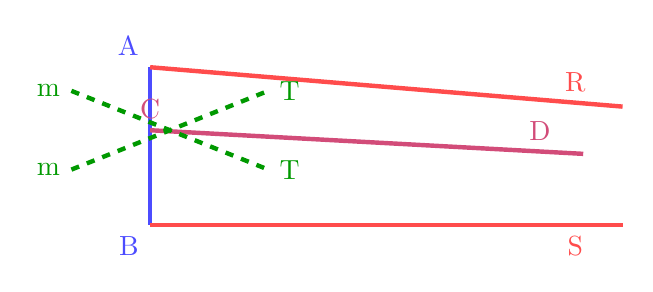
\begin{tikzpicture}[ultra thick]
	
	\coordinate (A) at (0,3);
	\coordinate (B) at (0,1);
	\coordinate (C) at (0,2.2);
	\coordinate (R) at (6,2.5);
	\coordinate (S) at (6,1);
	\coordinate (D) at (5.5,1.9);
	
	% Main vertical segment
	\draw[blue!70] (A) -- (B);
	
	% Outer sides
	\draw[red!70] (A) -- (R) node[pos=0.9, above, red!70] {R};
	\draw[red!70] (B) -- (S) node[pos=0.9, below, red!70] {S};
	
	% Middle segment
	\draw[purple!70] (C) -- (D) node[pos=0.9, above, purple!70] {D};
	
	% Dashed crossing lines
	\draw[dashed, green!60!black] (-1,2.7) -- (1.5,1.7) node[right, green!60!black] {T};
	\draw[dashed, green!60!black] (-1,1.7) -- (1.5,2.7) node[right, green!60!black] {T};
	
	% Labels for dashed lines
	\node[left, green!60!black] at (-1,2.7) {m};
	\node[left, green!60!black] at (-1,1.7) {m};
	
	% Point labels
	\node[above left, blue!70] at (A) {A};
	\node[below left, blue!70] at (B) {B};
	\node[above, purple!70] at (C) {C};
	
\end{tikzpicture}
\end{tasks*}
\end{proof}
	

\end{theorem}

\begin{theorem}
	\begin{tasks*}
		\item الزاوية الداخلية في مثلث محاذٍ (T.V.T) تكون أصغر من الزاوية الخارجية المقابلة لها.
		
		\item إذا كانت زاويتان في مثلثين محاذيين (T.V.T) متطابقتين على التوالي، فإن الأضلاع المقابلة لهما تكون متطابقة.
	\end{tasks*}
\end{theorem}

\textbf{ملاحظة:} في الهندسة الزائدية يكون مجموع زوايا أي مثلث أقل من $180^\circ$.

\begin{definition}[الانحراف المثلثي (Defect)]
	ليكن $\triangle ABC$ مثلثًا في الهندسة الهذلولية، فإن الانحراف المثلثي يُعرّف كما يلي:
	\[
	\mathrm{Defect}(\triangle ABC) = 180^\circ - (\angle A + \angle B + \angle C)
	\]
\end{definition}

\textbf{مثال:} أوجد الانحراف المثلثي لمثلث مجموع زواياه $150^\circ$.

\textbf{الحل:}
\[
\mathrm{Defect}(\triangle ABC) = 180^\circ - 150^\circ = 30^\circ
\]

\section[النسبة التبادلية]{النسبة التبادلية \cite{ref4}}

إذا كانت $A, B, C$ ثلاث نقاط على استقامة واحدة، فإن نسبة تقسيم قطعة المستقيم $AB$ بواسطة النقطة $C$، ويرمز لها بـ $(AB, C)$، تُعرّف كما يلي:
\[
(AB, C) = \frac{AC}{BC}
\]

\begin{itemize}[label*=\textbullet]
	\item إذا كانت النقطة $C$ تقع بين $A$ و$B$ فإن التقسيم يسمى \textbf{تقسيمًا داخليًا} وتكون النسبة سالبة، أما إذا كانت خارج القطعة فإن التقسيم يسمى \textbf{تقسيمًا خارجيًا} وتكون النسبة موجبة.
	\item $AB = -BA$
\end{itemize}


\begin{definition}[النسبة التبادلية (Cross-Ratio)]
	إذا كانت 
	$A(x_1, y_1), B(x_2, y_2), C(x_3, y_3), D(x_4, y_4)$ أربع نقاط على استقامة واحدة، فإن النسبة التبادلية لها تُعرّف كما يلي:
	\[
	(AB, CD) = \frac{(AB, C)}{(AB, D)} = \frac{(AC/BC)}{(AD/BD)} = \frac{(AC \cdot BD)}{(BC \cdot AD)} = \frac{(x_3 - x_1) \cdot (x_4 - x_2)}{(x_3 - x_2)\cdot(x_4 - x_1)}
	\]
	\begin{itemize}[label=\textbullet, leftmargin=*]
		\item اذا كانت $C\in AB$ و $D\in AB$ فأنه $(AB, CD)$ تكون موجبة.
		\item اذا كانت $C\in AB$ و $D\in AB$ فأنه $(AB, CD)$ تكون سالبة.
		
	\end{itemize}
\end{definition}
\begin{example}
	جد النسبة التبادلية للنقاط التالية
	\[
	A(1,1), \quad B(-2,-5), \quad C(3,5), \quad D(5,9)
	\]
	نحسب النسبة التبادلية \((AB,CD)\) باستخدام الصيغة:
	\[
	(AB,CD) = \frac{(x_3 - x_1)(x_4 - x_2)}{(x_3 - x_2)(x_4 - x_1)}
	 =\frac{(3-1)(5+2)}{(3+2)(5-1)} = \frac{2 \cdot 7}{5 \cdot 4} = \frac{14}{20} = \frac{7}{10}
	\]
\end{example}

\subsection*{بعض خواص النسبة التبادلية}
\begin{enumerate}
	\item $(AB, CD) = \frac{1}{(BA, CD)}$
	\item $(AB, CD) = \frac{1}{(AB, DC)}$
	\item $(AB, CD) = (CD, AB)$
	\item $(AB, CD) + (AC, BD) = 1$
\end{enumerate}

\section{المسافة بين نقطتين في الفضاء الهذلولي}

لإمكانية تصور أفكار الهندسة الزائدية نستعرض نموذج بوانكاريه لنصف المستوى العلوي (Poincaré Half-Plane Model)، حيث يتكون الفضاء من جميع النقاط $(X,Y)$ في المستوى بحيث:
\[
Y > 0
\]

\textbf{تعريف المستقيمات:}
تُعرّف المستقيمات في هذا النموذج على الشكل التالي:
\begin{enumerate}
	\item أنصاف الدوائر التي مراكزها على المحور $X$ وتقع في النصف العلوي.
	\item المستقيمات العمودية على المحور $X$ والمحصورة في $Y > 0$.
\end{enumerate}

\textbf{معادلة دائرة نموذجية:}
\[
Y = \sqrt{r^2 - (X - h)^2}
\]

والمستقيمات العمودية تعطى بالعلاقة:
\[
X = a, \quad Y > 0
\]

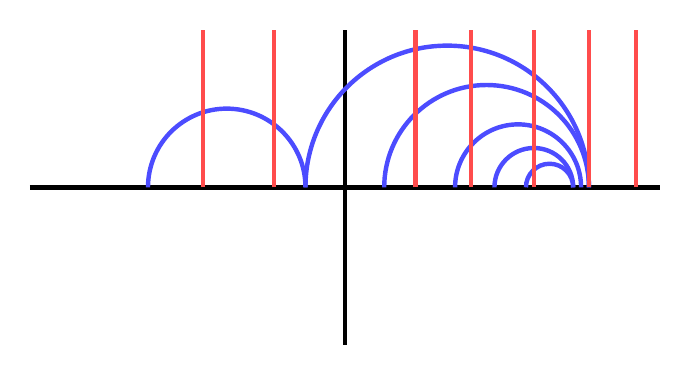
\begin{tikzpicture}[ultra thick]
	
	% Axes
	\draw[black] (-4,0) -- (4,0);
	\draw[black] (0,-2) -- (0,2);
	
	% Arcs (same family → same color)
	\draw[blue!70] (-2.5,0) arc (180:0:1);
	\draw[blue!70] (-0.5,0) arc (180:0:1.8);
	\draw[blue!70] (0.5,0) arc (180:0:1.3);
	\draw[blue!70] (1.4,0) arc (180:0:0.8);
	\draw[blue!70] (1.9,0) arc (180:0:0.5);
	\draw[blue!70] (2.3,0) arc (180:0:0.3);
	
	% Vertical lines
	\foreach \x in {-1.8, -0.9, 0.9, 1.6, 2.4, 3.1, 3.7} {
		\draw[red!70] (\x,0) -- (\x,2);
	}
	
\end{tikzpicture}

\noindent\textbf{المسافة الزائدية:}

تعرف المسافة الزائدية بين نقطتين $A$ و$B$ بأنها طول القوس من الدائرة التي تمر بالنقطتين ومركزها على المحور $X$، وتُعطى بالعلاقة:
\[
h(AB) = \frac{1}{2} \log \left( \frac{A'U \cdot B'V}{B'U \cdot A'V} \right)
\]

حيث تعتمد على النسبة التبادلية لأربع نقاط على المحور.

\textbf{ملاحظة:} إذا كان المستقيم عموديًا على المحور $X$ فإن المسافة تُعطى بـ:
\[
h(AB) = \log \left( \frac{UB}{UA} \right) = \log \left( \frac{b}{a} \right)
\]

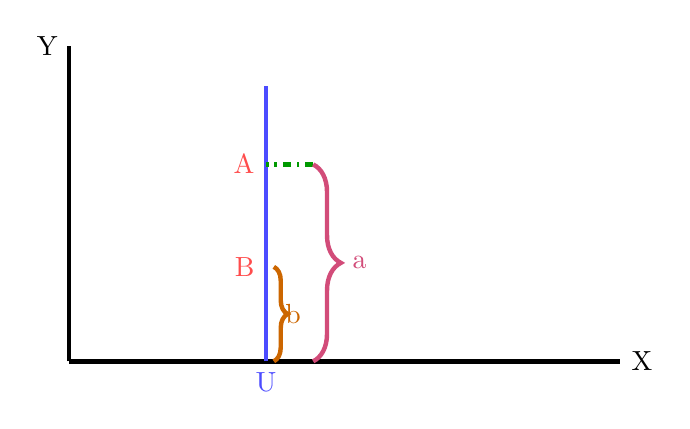
\begin{tikzpicture}[>=stealth, ultra thick]
	
	% Axes
	\draw[black] (0,0) -- (7,0) node[right] {X};
	\draw[black] (0,0) -- (0,4) node[left] {Y};
	
	% Vertical segment
	\coordinate (U) at (2.5,0);
	\draw[blue!70] (U) -- (2.5,3.5);
	\node[below, blue!70] at (U) {U};
	
	% Points
	\coordinate (A) at (2.5,2.5);
	\coordinate (B) at (2.5,1.2);
	
	\node[left, red!70] at (A) {A};
	\node[left, red!70] at (B) {B};
	
	% Small dashed marker
	\draw[dash pattern=on 3pt off 2pt on 1pt off 2pt, green!60!black] 
	(3.1,2.5) -- (2.5,2.5);
	
	% Braces (dimension indicators)
	\draw[decorate, decoration={brace, amplitude=10pt, mirror}, purple!70]
	(3.1,0) -- (3.1,2.5)
	node[midway, right, xshift=10pt, purple!70] {a};
	
	\draw[decorate, decoration={brace, amplitude=5pt, mirror}, orange!80!black]
	(2.6,0) -- (2.6,1.2)
	node[midway, right, orange!80!black] {b};
	
\end{tikzpicture}

\newpage
\begin{example}
	جد المسافة الهذلولية بين النقطتين 
	$A(\dfrac{1}{2}, \dfrac{\sqrt{3}}{2}), B(0,1)$
\end{example}
\begin{solution}
	نريد حساب المسافة الهذلولية بين النقطتين:
	\[
	A\left(\frac{1}{2}, \frac{\sqrt{3}}{2}\right), \quad B(0,1)
	\]
	\[
	h(AB) = \frac{1}{2}\log (A'B', UV) 
	\]
	حيث $U$ و $V$ نقطتا تقاطع الدائرة المارة بالنقطتين مع المحور $X$.

	لتكن معادلة الدائرة:
	\[
	(X - h)^2 + Y^2 = r^2
	\]
	\begin{otherlanguage}{english}
		\begin{figure}
			\centering
			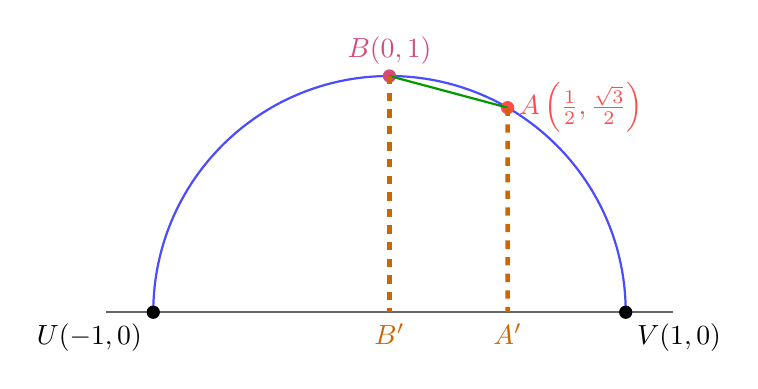
\begin{tikzpicture}[scale=3, ultra thick]
				
				% Semicircle and diameter
				\draw[blue!70, thick] (-1,0) arc(180:0:1);
				\draw[black!60, thick] (-1.2,0) -- (1.2,0);
				
				% Points
				\coordinate (A) at (0.5,0.866);
				\coordinate (B) at (0,1);
				\coordinate (U) at (-1,0);
				\coordinate (V) at (1,0);
				
				% Point markers + labels
				\fill[red!70] (A) circle (0.8pt)
				node[right, red!70] {$A\left(\frac{1}{2}, \frac{\sqrt{3}}{2}\right)$};
				
				\fill[purple!70] (B) circle (0.8pt)
				node[above, purple!70] {$B(0,1)$};
				
				\fill[black] (U) circle (0.8pt)
				node[below left] {$U(-1,0)$};
				
				\fill[black] (V) circle (0.8pt)
				node[below right] {$V(1,0)$};
				
				% Chord AB
				\draw[green!60!black, thick] (A) -- (B);
				
				% Projections
				\draw[dashed, orange!80!black] (A) -- (0.5,0)
				node[below, orange!80!black] {$A'$};
				
				\draw[dashed, orange!80!black] (B) -- (0,0)
				node[below, orange!80!black] {$B'$};
				
			\end{tikzpicture}
		\end{figure}
	\end{otherlanguage}	
	بالتعويض عن $A$:
	\[
	\left(\frac{1}{2} - h\right)^2 + \frac{3}{4} = r^2
	\]
	وبالتعويض عن $B$:
	\[
	h^2 + 1 = r^2
	\]
	بمساواة الطرفين:
	\[
	\left(\frac{1}{2} - h\right)^2 + \frac{3}{4} = h^2 + 1 \to \frac{1}{4} - h + h^2 + \frac{3}{4} = h^2 + 1 \to h = 0
	\]
	وبالتالي معادلة الدائرة:
	\[
	X^2 + Y^2 = 1
	\]
	اذن
	\begin{align*}
		h(AB) &= \frac{1}{2} \log\left[\frac{A'U\cdot B'V}{A'V\cdot B'U} \right]\\
		&= \frac{1}{2}\log\left[\frac{(-1-1/2)(1-0)}{(1 + 1/2)(-1-0)}\right]\\
		&=\frac{1}{2} \log \frac{1}{3}\\
		&= -\frac{1}{2} \log 3
	\end{align*}
\end{solution}

\section*{معادلة المستقيم الهذلولي الذي يمر بين نقطتين معلومتين}
	إذا كانت النقطتان $A(x_1,y_1)$ و $B(x_2,y_2)$ في نموذج بوانكاريه لنصف المستوى العلوي بحيث $x_1 \neq x_2$، فإن المستقيم الهذلولي المار بهما هو قوس دائرة يحقق معادلته:
	
	\[
	\begin{vmatrix}
		x^2 + y^2 & x & 1 \\
		x_1^2 + y_1^2 & x_1 & 1 \\
		x_2^2 + y_2^2 & x_2 & 1
	\end{vmatrix}
	= 0 \tag{1}
	\]
	
	حيث تمثل هذه العلاقة دائرة تمر بالنقطتين $A$ و $B$ ومركزها يقع على المحور $X$، وبالتالي يكون الجزء الواقع في $y>0$ هو المستقيم الهذلولي بينهما.

\begin{example}
	جد معادلة المستقيم الهذلولي المار بين النقطتين 
	$A( 1, 4 ), B(3, -2)$
\end{example}

\begin{solution}
	نريد إيجاد معادلة المستقيم الهذلولي المار بالنقطتين:
	\[
	A(1,4), \quad B(3,-2)
	\]
	حسب تعريف المستقيم الهذلولي في نموذج بوانكاريه (على شكل دائرة تمر بالنقطتين)، فإن معادلته تُعطى بالمحدد:
	\[
	\begin{vmatrix}
		x^2 + y^2 & x & 1 \\
		1^2 + 4^2 & 1 & 1 \\
		3^2 + (-2)^2 & 3 & 1
	\end{vmatrix}
	= 0
	\]
	إذن:
	\[
	\begin{vmatrix}
		x^2 + y^2 & x & 1 \\
		17 & 1 & 1 \\
		13 & 3 & 1
	\end{vmatrix}
	= 0
	\]
	\[
	(x^2 + y^2)\begin{vmatrix}1 & 1 \\ 3 & 1\end{vmatrix}
	- x \begin{vmatrix}17 & 1 \\ 13 & 1\end{vmatrix}
	+ 1 \begin{vmatrix}17 & 1 \\ 13 & 3\end{vmatrix}
	= 0
	\]
	\[
	-2(x^2 + y^2) - 4x + 38 = 0
	\]
	\[
	x^2 + y^2 + 2x - 19 = 0
	\]
\end{solution}
